\section{Einführung}

\begin{frame}
\frametitle{Einführung}
SL: typsicher und funktional im Browser (JavaScript)

\begin{center}
$\downarrow$
\end{center}

SL2: unabhängig kompilierbare Module

\begin{itemize}
\item Moduldefinition und -import (auch für das Prelude)
\item Export und einfache Qualifizierung von Funktionen und
    Datentypen
\item Einbindung von Funktionen und Datentypen aus JavaScript
\item Anpassungen der Syntax und Semantik
\item Fehlermeldungen verbessert
\item Compilierung ins Dateisystem
\item Bibliotheken, Beispielprogramme und Tests
\end{itemize}
\end{frame}

\begin{frame}
\frametitle{Altes Framework}

\begin{figure}
\center{%
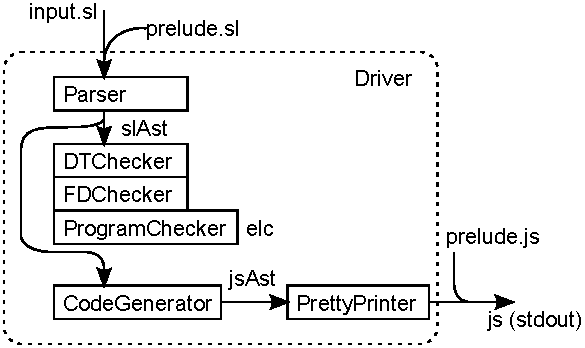
\includegraphics[width=1\linewidth]{programFlowOld}}
\end{figure}

\end{frame}

\begin{frame}
\frametitle{Neues Framework}

\begin{figure}
\center{%
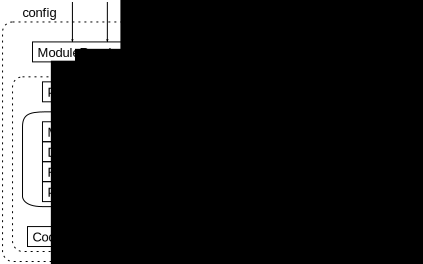
\includegraphics[width=1\linewidth]{programFlow}}
\end{figure}

\end{frame}
